% Two-panel schematic: replacement vs mutual interchange (central contrast).
% Skip-layer removal is defined in the main text and evaluated in the skip-layer PPL tables.
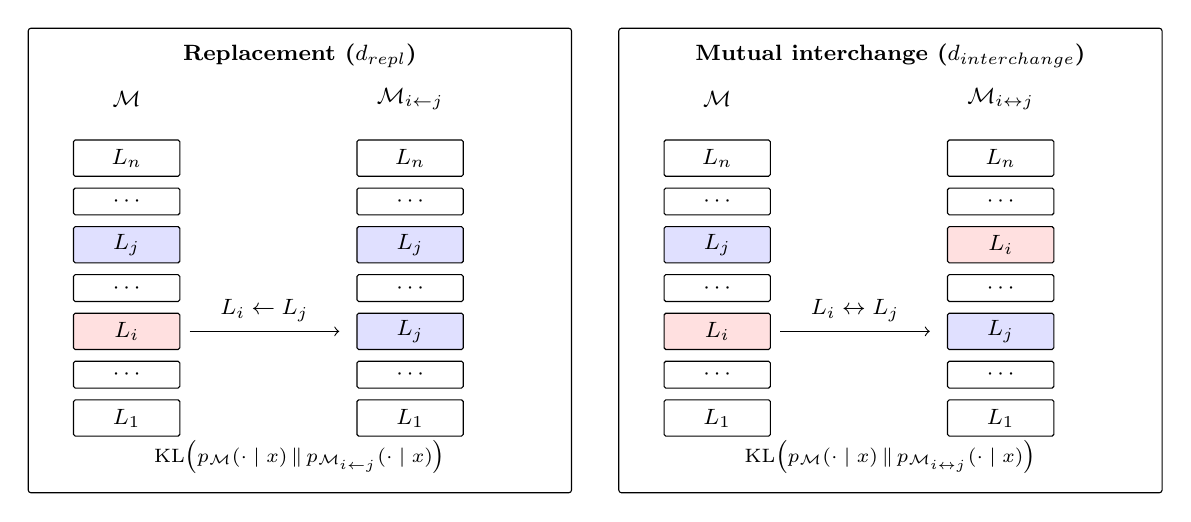
\begin{tikzpicture}[font=\footnotesize, line width=0.4pt]
\tikzset{
    layer/.style={draw, rounded corners=0.6pt, minimum width=1.35cm, minimum height=0.46cm, inner sep=2pt, align=center},
    dots/.style={draw, rounded corners=0.6pt, minimum width=1.35cm, minimum height=0.34cm, inner sep=2pt, align=center},
    layeri/.style={layer, fill=red!12},
    layerj/.style={layer, fill=blue!12}
}

% Panel frames
\draw[rounded corners=1pt] (0,0) rectangle (6.9,5.9);
\draw[rounded corners=1pt] (7.5,0) rectangle (14.4,5.9);
\node[font=\bfseries\footnotesize] at (3.45,5.55) {Replacement ($d_{\text{repl}}$)};
\node[font=\bfseries\footnotesize] at (10.95,5.55) {Mutual interchange ($d_{\text{interchange}}$)};

% --- Left: replacement ---
\node at (1.25,5.0) {$\mathcal{M}$};
\node at (4.85,5.0) {$\mathcal{M}_{i\leftarrow j}$};

\node[layer]  at (1.25,0.95) {$L_1$};
\node[dots]   at (1.25,1.50) {$\cdots$};
\node[layeri] at (1.25,2.05) {$L_i$};
\node[dots]   at (1.25,2.60) {$\cdots$};
\node[layerj] at (1.25,3.15) {$L_j$};
\node[dots]   at (1.25,3.70) {$\cdots$};
\node[layer]  at (1.25,4.25) {$L_n$};

\node[layer]  at (4.85,0.95) {$L_1$};
\node[dots]   at (4.85,1.50) {$\cdots$};
\node[layerj] at (4.85,2.05) {$L_j$};
\node[dots]   at (4.85,2.60) {$\cdots$};
\node[layerj] at (4.85,3.15) {$L_j$};
\node[dots]   at (4.85,3.70) {$\cdots$};
\node[layer]  at (4.85,4.25) {$L_n$};

\draw[->] (2.05,2.05) -- (3.95,2.05) node[midway,above] {$L_i \leftarrow L_j$};
\node[font=\scriptsize] at (3.45,0.45) {$\mathrm{KL}\!\left(p_{\mathcal{M}}(\cdot\mid x)\,\|\,p_{\mathcal{M}_{i\leftarrow j}}(\cdot\mid x)\right)$};

% --- Right: mutual interchange ---
\node at (8.75,5.0) {$\mathcal{M}$};
\node at (12.35,5.0) {$\mathcal{M}_{i \leftrightarrow j}$};

\node[layer]  at (8.75,0.95) {$L_1$};
\node[dots]   at (8.75,1.50) {$\cdots$};
\node[layeri] at (8.75,2.05) {$L_i$};
\node[dots]   at (8.75,2.60) {$\cdots$};
\node[layerj] at (8.75,3.15) {$L_j$};
\node[dots]   at (8.75,3.70) {$\cdots$};
\node[layer]  at (8.75,4.25) {$L_n$};

\node[layer]  at (12.35,0.95) {$L_1$};
\node[dots]   at (12.35,1.50) {$\cdots$};
\node[layerj] at (12.35,2.05) {$L_j$};
\node[dots]   at (12.35,2.60) {$\cdots$};
\node[layeri] at (12.35,3.15) {$L_i$};
\node[dots]   at (12.35,3.70) {$\cdots$};
\node[layer]  at (12.35,4.25) {$L_n$};

\draw[->] (9.55,2.05) -- (11.45,2.05) node[midway,above] {$L_i \leftrightarrow L_j$};
\node[font=\scriptsize] at (10.95,0.45) {$\mathrm{KL}\!\left(p_{\mathcal{M}}(\cdot\mid x)\,\|\,p_{\mathcal{M}_{i \leftrightarrow j}}(\cdot\mid x)\right)$};
\end{tikzpicture}
